\documentclass[10pt]{article}
\usepackage[margin=1in]{geometry}
\usepackage{parskip}
\usepackage{microtype}
\usepackage[square]{natbib}
\usepackage{graphicx}
\usepackage{amsmath}
% \usepackage{txfonts}
\usepackage[font=small,labelfont=bf]{caption}

\graphicspath{ {figures/} }
\linespread{1.3}


\begin{document}

\title{Distinguishing NFW and Isothermal Density Profiles with Weak Gravitational Lensing}
\author{Ian Holst and Doyee Byun}
\date{\today}
\maketitle

\begin{abstract}
We examine the feasibility of distinguishing NFW and cored isothermal density profiles using weak gravitational lensing shear.

We model lenses in the two different profiles, as well as background galaxies to be lensed.
Analyzing the simulated data of these lensed galaxies gives us insight into how we can distinguish the differences between the two profiles.
This method is expected to be helpful in the analysis of real observation data in the future.
\end{abstract}


\section{Introduction}
Gravitational lensing allows us to investigate the matter density distributions of cosmic objects by observing the characteristic light distortions imparted on other objects in the background. The principle is applicable on a large range of scales, from all-sky mass maps based on cosmic microwave background shear, to studies of individual galaxies and clusters. In particular, by observing the coherent distortions of many background galaxies, the shear profile, and consequently the density profile of a foreground halo lens may be determined.

Two commonly used density profiles in the field are the isothermal profile and the Navarro-Frenk-White (NFW) profile. The NFW profile has been found to fit simulated dark matter halos very well \citep{}, while the isothermal profile results from an idealized isothermal collapse \citep{}. Both profiles extend to infinity

It is of great interest to determine the general forms of halo density profiles
since this tells us about structure formation and the nature of dark matter
\citep{}
Lensing offers one of the few ways to probe the distribution of all matter, not just baryonic matter.
rotation curve present difficulties (https://arxiv.org/pdf/astro-ph/0201352.pdf)

In this paper, we will investigate the distinguishability of NFW and isothermal profiles
given galaxy-galaxy lensing data
The goal of this project is to devise a method to analyze lensed galaxy cluster data and find which density profile is more probable between the isothermal and NFW profiles.
In order to do so, we generate simulated data sets and analyze them to find the more probable profiles they would fit into.
This analysis method is expected to be usable in determining the characteristics of real observed data as well.


Outline:
We start by introducing the general lensing characteristics of spherical density profiles, followed by the specifics for cored isothermal and NFW profiles. We then describe
The results


\subsection{Lensing by a spherical lens profile}
Here we define our conventions for various lensing quantities, which mainly conform to those used by \citet{Dodelson2017}. We use the thin lens approximation and assume spherical lens profiles. Consider such a spherically symmetric halo density profile $\rho(r)$ acting as a gravitational lens. This lens halo is located at an angular diameter distance $D_L$ from the observer and we want to find out how it affects a source object behind it at an angular diameter distance $D_S$. Set the $z$ axis to be along the line of sight, and use local cylindrical coordinates $R$, $\phi$, and $z$. The projected surface density $\Sigma$ at radius $R$ on the projected plane is obtained by integrating the density over the entire $z$ axis:
\begin{equation} \label{sigma}
\Sigma(R) = \int_{-\infty}^{\infty}{dz\ \rho(\sqrt{R^2 + z^2})}
\end{equation}
A useful related measure in gravitational lensing is the average projected surface density within a radius $R$:
\begin{equation} \label{sigmabar}
\overline{\Sigma}(R) = \frac{1}{\pi R^2} \int_0^{2\pi}{d\phi \int_0^{R}{dR'~\Sigma(R')R'}}
\end{equation}
The critical surface density is an important quantity that marks the typical boundary between what is considered strong and weak lensing:
\begin{equation} \label{sigmacrit}
\Sigma_\mathrm{crit} = \frac{c^2}{4\pi G} \frac{D_S}{D_{SL} D_L}
\end{equation}

$D_S$ and $D_L$ are calculated like normal angular diameter distances in a flat expanding universe: $D = \chi(z)/(1 + z)$, where $\chi(z)$ is the comoving distance to redshift $z$. The redshift $z$ of an object, such as a halo lens or a background galaxy, is typically easy to measure. Note that $D_{SL}$ is nominally the distance from the source to the lens, but since it is an angular diameter distance, it is calculated as $D_{SL} = (\chi_S - \chi_L)/(1 + z_S)$.

All relevant angles in this problem are small, so we can assume that $R = D_L \theta$, where $\theta$ is the angular position on the observer's sky, with the halo center at the origin. This may be represented as the vector $\vec{\theta}$, but in the spherically symmetric case, the magnitude $\theta$ is sufficient. Thus we can easily change variables in all lensing quantities from $R$ to $\theta$.

We define the convergence $\kappa$ at angular position $\theta$ as the ratio of surface density to critical surface density. Strong lensing phenomena such as arcs, rings, multiple images, and magnification are dominant when the convergence is greater than 1, or the projected surface density is greater than the critical surface density.
\begin{equation} \label{convergence}
\kappa(\theta) = \frac{\Sigma(\theta)}{\Sigma_\mathrm{crit}}
\end{equation}
While the convergence determines how an object is uniformly scaled or magnified by a gravitational lens, another quantity, shear, describes the stretching of images along an axis. Shear is usually expressed as two components, $\gamma_1$ and $\gamma_2$. The tangential shear $\gamma_t$ is the component of stretching in the $\hat{\phi}$ direction. It can be shown that for a spherical lens profile, the only component of shear $\gamma$ should be the tangential shear, $\gamma_t$. For a spherical lens, tangential shear can be shown to be simply related to the convergence and average convergence \citep{Dodelson2017}:
\begin{equation} \label{tangentialshear}
\gamma_t(\theta) = \overline{\kappa}(\theta) - \kappa(\theta)
\end{equation}
The tangential shear is decomposed into two components, $\gamma_1$ and $\gamma_2$. $\gamma_1$ represents stretching along the $\theta_x$ and $\theta_y$ axes, and $\gamma_2$ represents stretching along the $\theta_y = \theta_x$ and $\theta_y = - \theta_x$ lines. They can be obtained through a relation with $\gamma_t$ and the cylindrical azimuthal angle $\phi$.
\begin{equation}
\begin{split}
\gamma_1 = -\gamma_t \cos{2\phi}\\
\gamma_2 = -\gamma_t \sin{2\phi}
\end{split}
\end{equation}
The shear magnitude, which is equal to tangential shear, also follows from trigonometric identities:
\begin{equation}
\gamma = \gamma_t = -\gamma_1 \cos{2\phi} -\gamma_2 \sin{2\phi}
\end{equation}

Changes in object shapes due to lensing can be quantified using the ellipticity $\epsilon$. This is most commonly used in weak lensing, where shape changes are best described by simple stretching. Ellipticity is defined using the semimajor axis $a$ and semiminor axis $b$ of an ellipse \citep{Narayan1996}:
\begin{equation}
\epsilon = \frac{a^2 - b^2}{a^2 + b^2}
\end{equation}
Like shear, there are two components of ellipticity, $\epsilon_1$ and $\epsilon_2$, which are analogous to the shear components $\gamma_1$ and $\gamma_2$. The ellipticity that would be induced in an otherwise perfectly circular object is:
\begin{equation} \label{ellipticity}
\epsilon_i = \frac{2 \gamma_i/(1 - \kappa)}{1 + \gamma^2/(1 - \kappa)^2}
\end{equation}
And there is an analogous ellipticity magnitude or tangential ellipticity:
\begin{equation}
\epsilon =  -\epsilon_1 \cos{2\phi} -\epsilon_2 \sin{2\phi}
\end{equation}

Gravitational lensing causes a deflection in the observed image position of background objects. If the true position of the object is $\vec{\beta}$ and it appears at position $\vec{\theta}$, then the deflection angle is defined:
\begin{equation}
\vec{\alpha}(\vec{\theta}) = \overline{\kappa}(\theta)\vec{\theta}
\end{equation}
From this expression, it can be seen that deflection is most significant in the strong lensing regime, where $\kappa > 1$.


\subsection{Cored Isothermal Sphere Profile}

The cored isothermal sphere (CIS) profile is related to the singular isothermal sphere (SIS) profile, which is often used to describe halos and other collapsed astrophysical objects because of its simple formulation. Unlike the singular isothermal sphere, the cored isothermal sphere does not have a density singularity at its center due to a finite core radius $r_c$. The CIS density profile is defined
\begin{equation} \label{cisdensity}
\rho_\mathrm{CIS}(r) = \frac{\sigma^2}{2\pi G (r^2 + {r_c}^2)},
\end{equation}
where $\sigma^2$ is the velocity dispersion of the halo \citep{Chen2005, Shapiro1999}. Applying equation \ref{sigma} and defining $\theta_c = r_c/D_L$, we get the projected surface density of the CIS profile:
\begin{equation}
\Sigma_\mathrm{CIS}(\theta) = \frac{\sigma^2}{2 G D_L \sqrt{\theta^2 + {\theta_c}^2}}
\end{equation}
The average surface density inside angular radius $\theta$ is derived using equation \ref{sigmabar}:
\begin{equation}
\overline{\Sigma}_\mathrm{CIS}(\theta) = \frac{\sigma^2 \left(\sqrt{\theta^2 + {\theta_c}^2} - \theta_c \right)}{G D_L \theta^2}
\end{equation}
The tangential shear follows from equation \ref{tangentialshear}:
\begin{equation}
\gamma_\mathrm{CIS}(\theta) = \frac{\sigma^2}{\Sigma_\mathrm{crit} G D_L} \left(\frac{\sqrt{\theta^2 + {\theta_c}^2} - \theta_c}{\theta^2} - \frac{1}{2 \sqrt{\theta^2 + {\theta_c}^2}}\right)
\end{equation}
The ellipticity equation, while not quite elegant, is trivial to calculate using equation \ref{ellipticity}. Figure \ref{cisproperties} shows the convergence, tangential shear, and ellipticity of a Milky Way-sized halo lens.

\begin{figure}
    \centering
    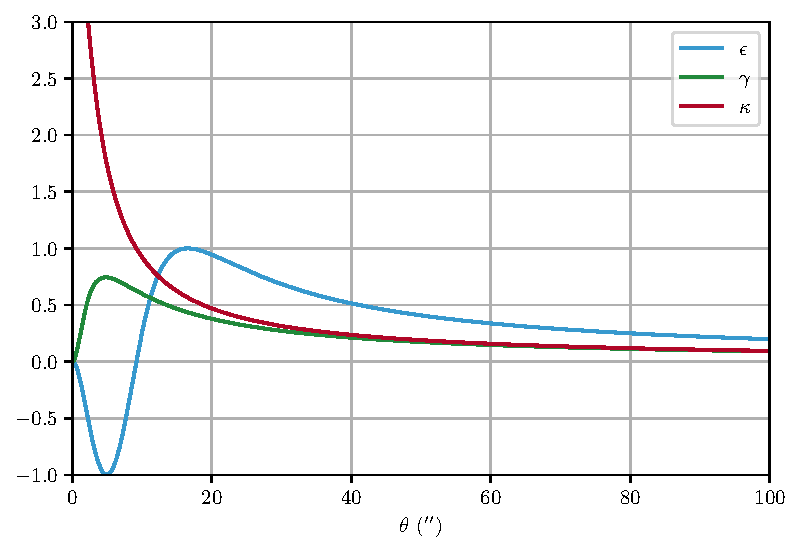
\includegraphics[width=0.8\textwidth]{isothermalproperties.pdf}
    \caption{Lensing quantities for a CIS profile with $M_{200} = 10^{15} M_\odot$ and $r_c = 10$ kpc. $z_L = 0.3$ and $z_S = 1.0$.}
    \label{cisproperties}
\end{figure}

Although the total mass of the CIS profile diverges, we will use a common convention for quantifying the mass of the profile within a reasonable radius. We define $r_{200}$ as the radius at which the average enclosed density of the profile is 200 times the critical density of the universe. The critical density $\rho_\mathrm{crit}$ depends on cosmological parameters such as the Hubble constant $H_0$. We choose to use the critical density at the current time $\rho_\mathrm{crit,0}$ for all halos regardless of their redshift. We assume a flat $\Lambda$CDM universe and use the Planck 2015 results for all cosmological calculations \citep{PlanckCollaboration2015}.

We define $M_{200}$ as the total mass enclosed within $r_{200}$:
\begin{equation} \label{M200}
M_{200} = 200 \rho_\mathrm{crit} \frac{4}{3} \pi {r_{200}}^3
\end{equation}
We also calculate $M_{200}$ specifically for a CIS profile by integrating equation \ref{cisdensity}:
\begin{equation} \label{cisM200}
M_{200} = M_\mathrm{enc}(r_{200}) = \frac{2 \sigma^2}{G} \left( r_{200} - r_c \arctan{\left(\frac{r_{200}}{r_c}\right)} \right)
\end{equation}
Solving for $r_{200}$:
\begin{equation} \label{r200}
r_{200} = \left( \frac{3 M_{200}}{800 \pi \rho_\mathrm{crit}} \right)^{1/3}
\end{equation}
We can now completely switch the CIS profile's dependence from $\sigma^2$ to $M_{200}$ with equation \ref{r200} and solving for $\sigma^2$ from equation \ref{cisM200}:
\begin{equation}
\sigma^2 = \frac{M_{200} G}{2 \left( r_{200} - r_c \arctan{\left(\frac{r_{200}}{r_c}\right)} \right)}
\end{equation}


\subsection{Navarro-Frenk-White (NFW) Profile} \label{nfwsection}
The NFW profile has had some success in describing dark matter halos in both simulations and observations \citep{Navarro1997}. It is characterized by a scale radius $r_s$ and a dimensionless parameter $\delta_c$, sometimes called the characteristic overdensity \citep{Wright2000}. It also depends on the critical density of the universe, which we evaluate at the current time, like before. The form of the NFW profile is:
\begin{equation}
\rho_\mathrm{NFW}(r) = \frac{\rho_\mathrm{crit} \delta_c}{(r/r_s)\left(1 + r/r_s\right)^2}
\end{equation}
Applying equation \ref{sigma} and defining $\theta_c = r_c/D_L$, we get the projected surface density of the NFW profile:
\begin{equation} \label{sigmanfw}
\Sigma_\mathrm{NFW}(\theta) = \frac{2 \rho_\mathrm{crit} \delta_c D_L \theta_s}{(\theta/\theta_s)^2 - 1} \left(1 - \frac{2}{\sqrt{(\theta/\theta_s)^2 - 1}} \arctan\left(\sqrt{\frac{\theta/\theta_s - 1}{\theta/\theta_s + 1}} \right) \right)
\end{equation}
\citet{Wright2000} use a slightly different convention for the projected surface density of an NFW profile. Note that for $\theta < \theta_s$, the argument of the arctan function in equation \ref{sigmanfw} becomes imaginary. However, applying the identity $\arctan(i x) = i\ \mathrm{arctanh}(x)$ and dividing out the $i$ from the square root in the denominator results in the form of $\Sigma_\mathrm{NFW}$ suggested by Wright and Brainerd for when  $\theta < \theta_s$. Additionally, their $\theta = \theta_s$ case is just the limit of equation \ref{sigmanfw} when $\theta \rightarrow \theta_s$. We argue that all three cases presented are equivalent and therefore we only use one for simplicity. \citet{Bartelmann2001} also use our convention.

The average surface density of an NFW profile is:
\begin{equation} \label{sigmabarnfw}
\overline{\Sigma}_\mathrm{NFW}(\theta) = \frac{4 \rho_\mathrm{crit} \delta_c D_L \theta_s}{(\theta/\theta_s)^2} \left(
    \frac{2}{\sqrt{(\theta/\theta_s)^2 - 1}} ~\arctan\left(\sqrt{\frac{\theta/\theta_s - 1}{\theta/\theta_s + 1}} \right) + \ln{\left(\frac{\theta/\theta_s}{2}\right)}
\right)
\end{equation}

The equations for tangential shear and ellipticity of an NFW profile are very cumbersome but follow trivially from equations \ref{tangentialshear}, \ref{ellipticity}, \ref{sigmanfw}, and \ref{sigmabarnfw}. Figure \ref{nfwproperties} shows the convergence, tangential shear, and ellipticity of a typical Milky Way-sized NFW halo lens.

\begin{figure}
    \centering
    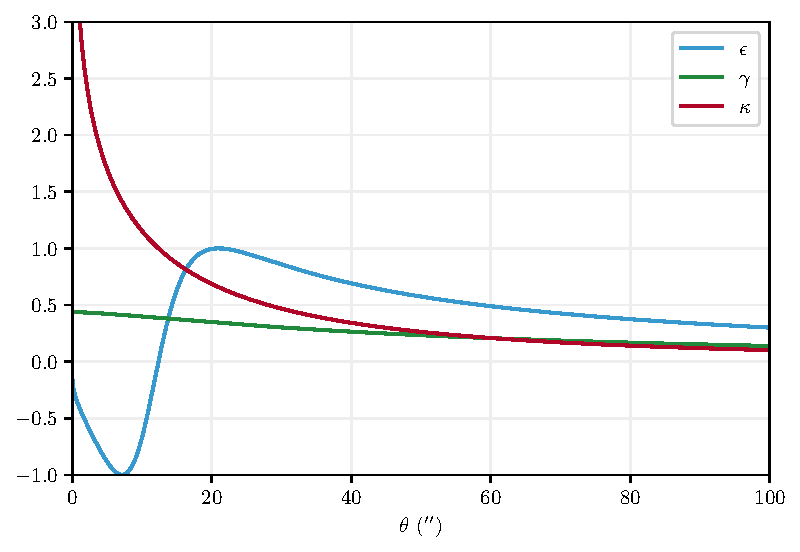
\includegraphics[width=0.8\textwidth]{nfwproperties.pdf}
    \caption{Lensing quantities for a NFW profile with $M_{200} = 10^{15} M_\odot$ and $c = 10$. Also,  $z_L = 0.3$ and $z_S = 1.0$.}
    \label{nfwproperties}
\end{figure}

Like the CIS profile, we would like to switch dependence to $M_{200}$ and the concentration parameter $c$ from $r_s$ and $\delta_c$. The concentration parameter $c$ is defined as the ratio of $r_{200}$ to the scale radius $r_s$:
\begin{equation} \label{concentration}
c = \frac{r_{200}}{r_s}
\end{equation}
By integrating the NFW density profile spherically out to radius $r_{200}$, we get the form of $M_{200}$:
\begin{equation} \label{nfwM200}
M_{200} = M_\mathrm{enc}(r_{200}) = 4 \pi \rho_\mathrm{crit} \delta_c {r_s}^3 \left( \frac{1}{1 + r_{200}/r_s} + \ln{\left(1 + \frac{r_{200}}{r_s} \right)} - 1 \right)
\end{equation}
Setting this equal to the definition of $M_{200}$ in equation \ref{M200}, substituting $c$ for $r_{200}$ using equation \ref{concentration}, and solving for $\delta_c$ gives:
\begin{equation}
\delta_c = \frac{200}{3} \frac{c^3}{\ln(1 + c) - c/(1 + c)}
\end{equation}
$r_s$ can be eliminated with equations \ref{concentration} and \ref{M200}.


\section{Methods}
In order to test the distinguishability of CIS and NFW profiles via gravitational lensing shear, we model a lensing scenario with one foreground lens and many background galaxies with random positions and intrinsic ellipticities. We calculate the effects of the lens on the shapes of the background galaxies to generate a dataset similar to what one might observe in reality. We then attempt to fit both CIS and NFW profiles to the data to see if there is a clear preference for the profile used to generate the data. We use the Planck 2015 results for all cosmological parameters \citep{PlanckCollaboration2015}.

\subsection{Simulated Data Generation}
We model a single foreground lens halo with an NFW profile using the equations derived in section \ref{nfwsection}. The profile has $M_{200} = 10^{15} M_\odot$ and $c = 10$, which are typical values for a Milky Way-sized dark matter halo. The lens is placed at redshift $z_L = 0.3$, which is comparable to that of the Bullet Cluster, an interesting lensing target \citep{Clowe2006}.

We generate a field of background galaxies within a 1000 arcsecond by 1000 arcsecond square centered on the lens. The number of galaxies is chosen so that the average angular number density is 50 galaxies per square arcminute, which is an optimistic expectation for the observing capability of the Large Synoptic Survey Telescope (LSST) \citep{Chang2013}. The $(\theta_x, \theta_y)$ coordinates of each background galaxies are generated randomly within the range of the field. The intrinsic contributions to the ellipticity components $\epsilon_1$ and $\epsilon_2$ are also randomly sampled from a Gaussian distribution with mean $\mu_\epsilon = 0$ and standard deviation $\sigma_\epsilon = 0.2$. This is consistent with the findings of \citet{Niemi2015} from observations. We place all galaxies at the same redshift $z_S = 1.0$, which is comparable to many objects in the Hubble Deep Field. This is justified because redshift can be simple to determine and account for when analyzing lensing in observational data.

We apply lensing shear to all the background galaxies based on their distance from the center of the halo, assuming that ellipticities add together linearly. We neglect the application of deflection angles since this would have little effect on fitting, and shear is derived as a function of image position rather than source position. Effectively, we assume all galaxies are already at their deflected position. Also, the majority of the background galaxies lie in the weak lensing regime, where the deflection angle can be negligible. The result is a simulated dataset with $N$ galaxies, and $N$ corresponding sets of  $\{\theta_x, \theta_y, \epsilon_1, \epsilon_2\}$.

Figure \ref{ellipticityexample} illustrates the effects of shear by both CIS and NFW profiles on a background galaxy field. The galaxy number density is exaggerated in comparison to the one used to generate data for actual analysis. The strong lensing regime is apparent near the center, where tangential ellipticity is negative and there is an impression of critical curves (compare to figures \ref{cisproperties} and \ref{nfwproperties}). The two profiles are nearly impossible to distinguish by eye, but precise data and statistics will offer a different picture.

\begin{figure}
    \centering
    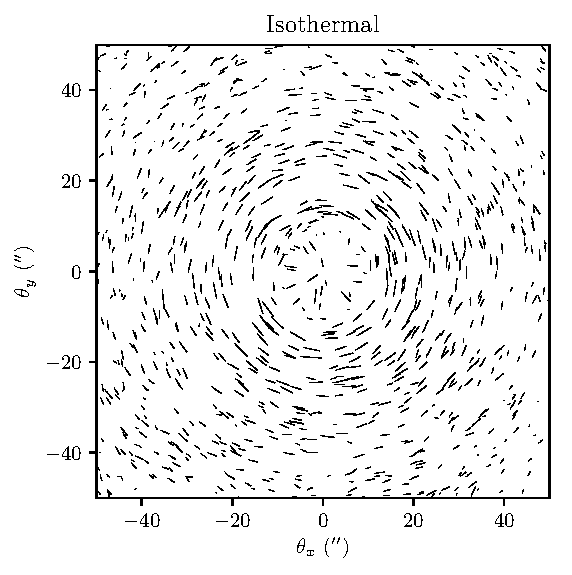
\includegraphics[width=0.49\textwidth]{isothermalellipticities.pdf}
    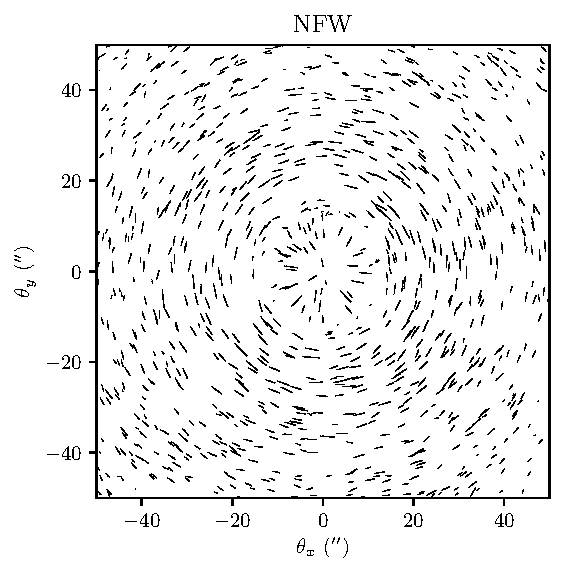
\includegraphics[width=0.49\textwidth]{nfwellipticities.pdf}
    \caption{Simulated lensing of a field of background galaxies by a CIS lens (left) and NFW lens (right). Each line represents a single galaxy. Intrinsic ellipticities are drawn from a Gaussian distribution of mean 0 and standard deviation 0.2. The length of the line indicates the post-lensing ellipticity, while the orientation represents the direction that the galaxy is sheared.}
    \label{ellipticityexample}
\end{figure}


\subsection{Data Analysis and Fitting}
To reconstruct a shear profile of the lens, we bin the galaxies into 40 linearly spaced annuli by their $\theta$ magnitude. The bins extend from from 10" out to approximately 700". Within each bin, we
and form a

Calculate mean and standard deviation of ellipticity
Attempt to fit both NFW and isothermal profiles, see if the fit is distinguishable


we fit expressions for ellipticity

We fit by numerically minimizing $\chi^2$
\begin{equation}
\chi^2 =
\end{equation}

%What theta range should we look at? (5 arcminutes?)

%How to properly do sigma contours?

\section{Results}
The parameter fitting results are as shown in figures.

\begin{figure}
    \centering
    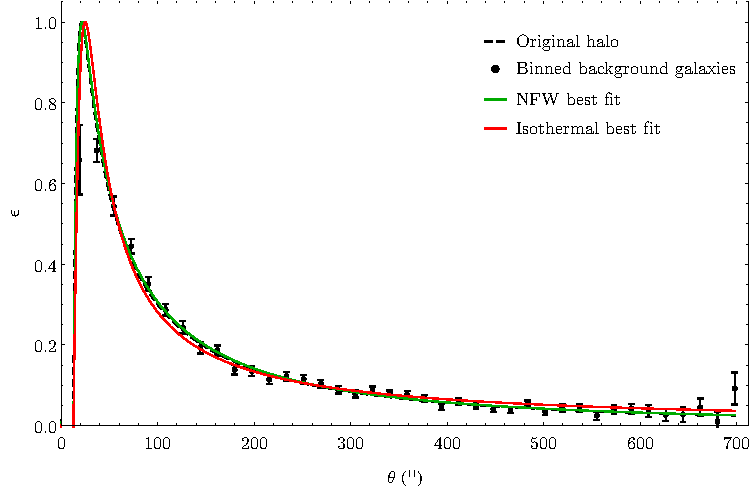
\includegraphics[width=0.9\textwidth]{comparison.pdf}
    \caption{plots}
    \label{}
\end{figure}

% \begin{figure}
%     \centering
%     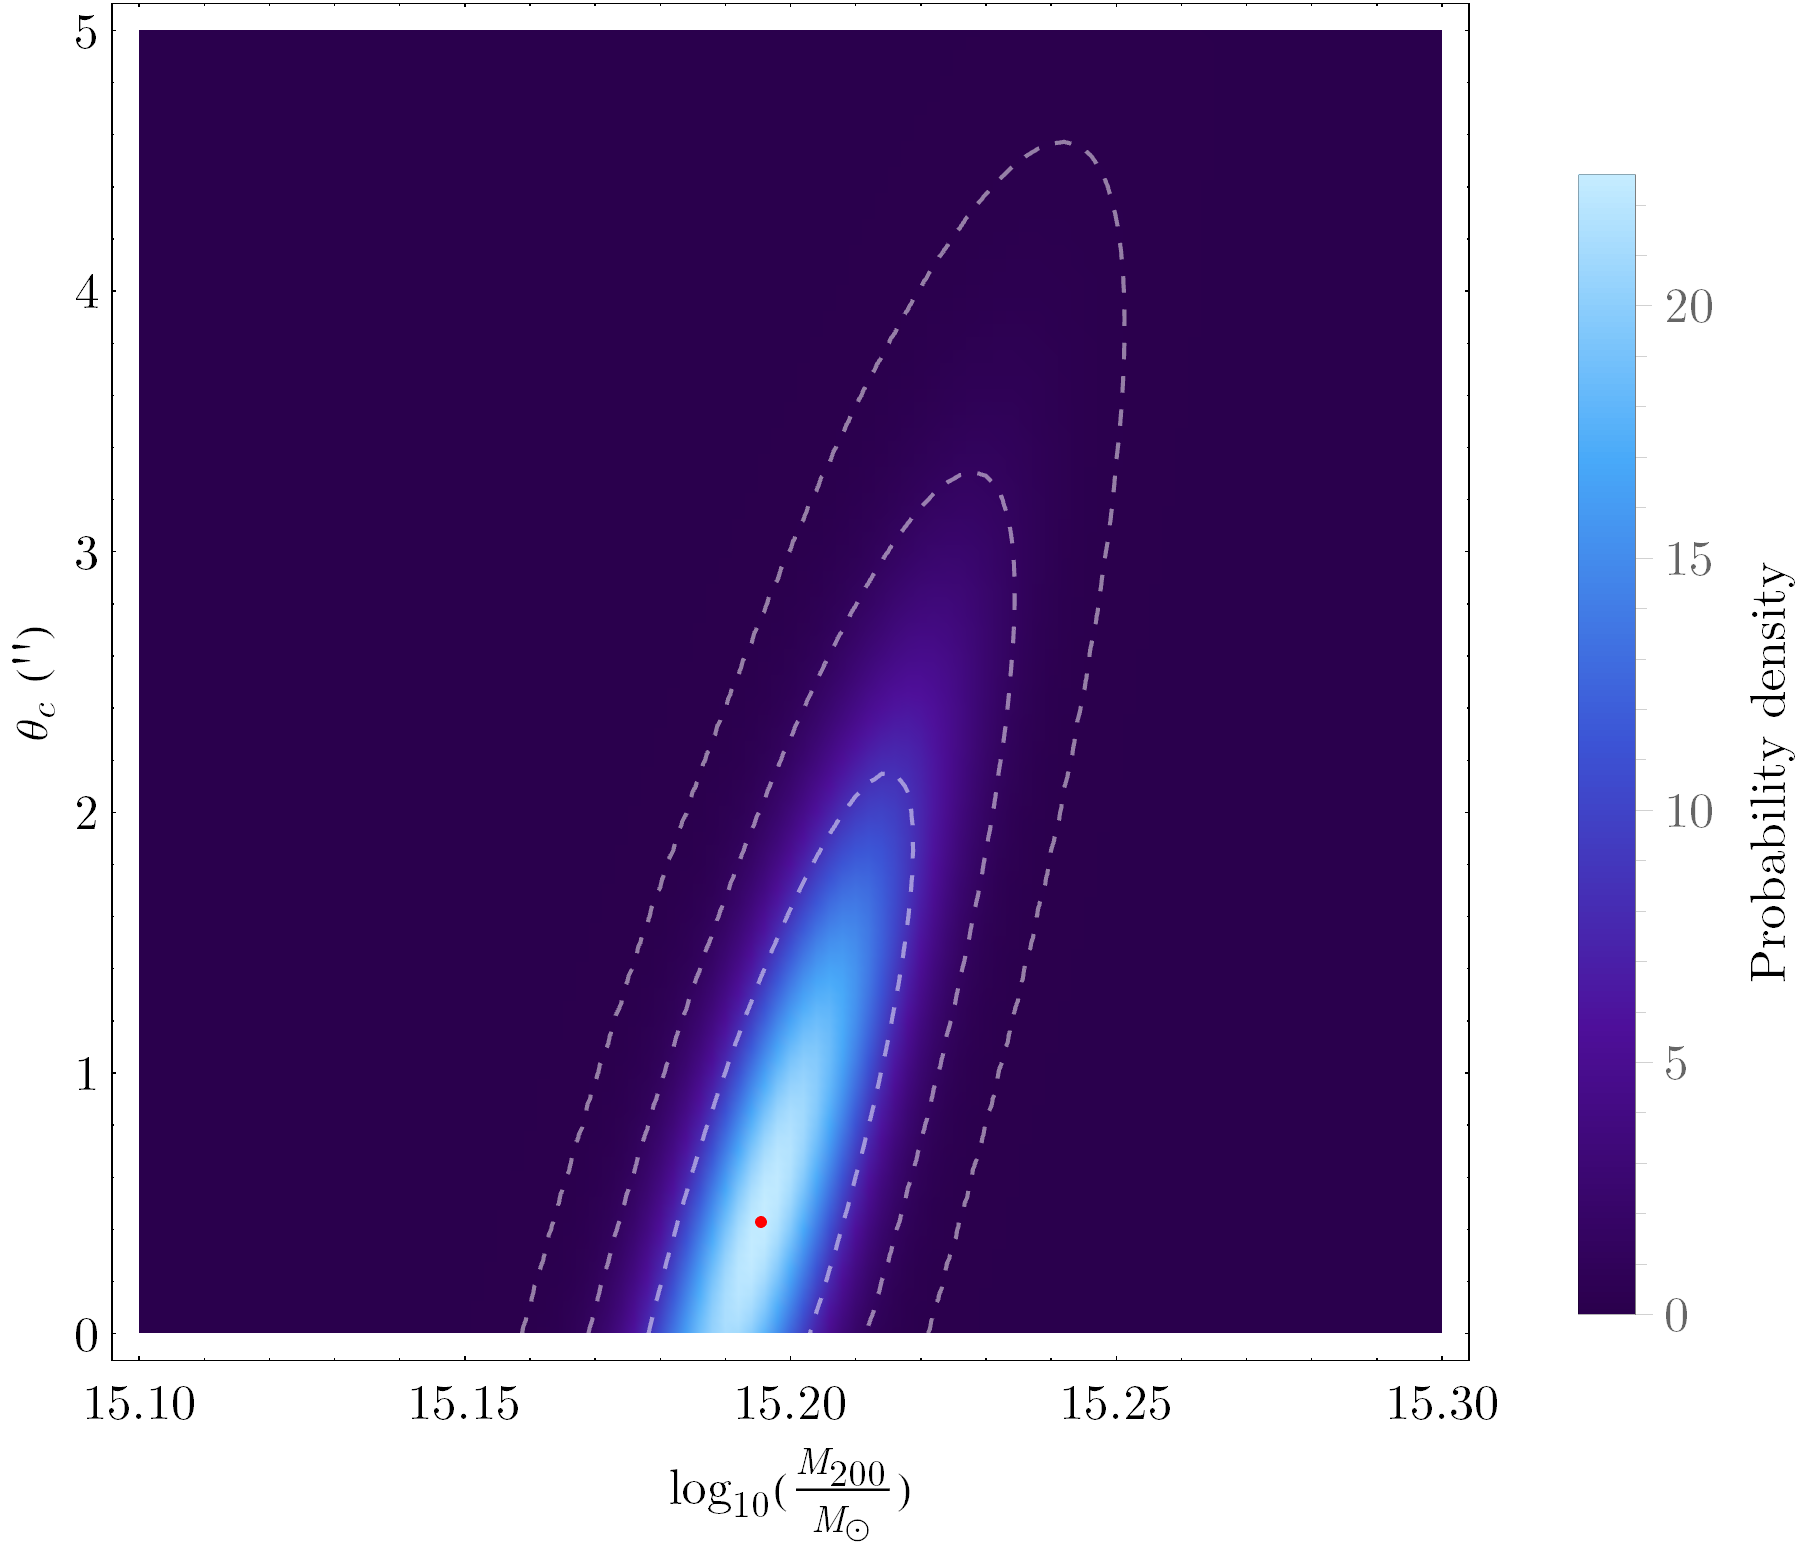
\includegraphics[width=0.49\textwidth]{isothermalfitparams.pdf}
%     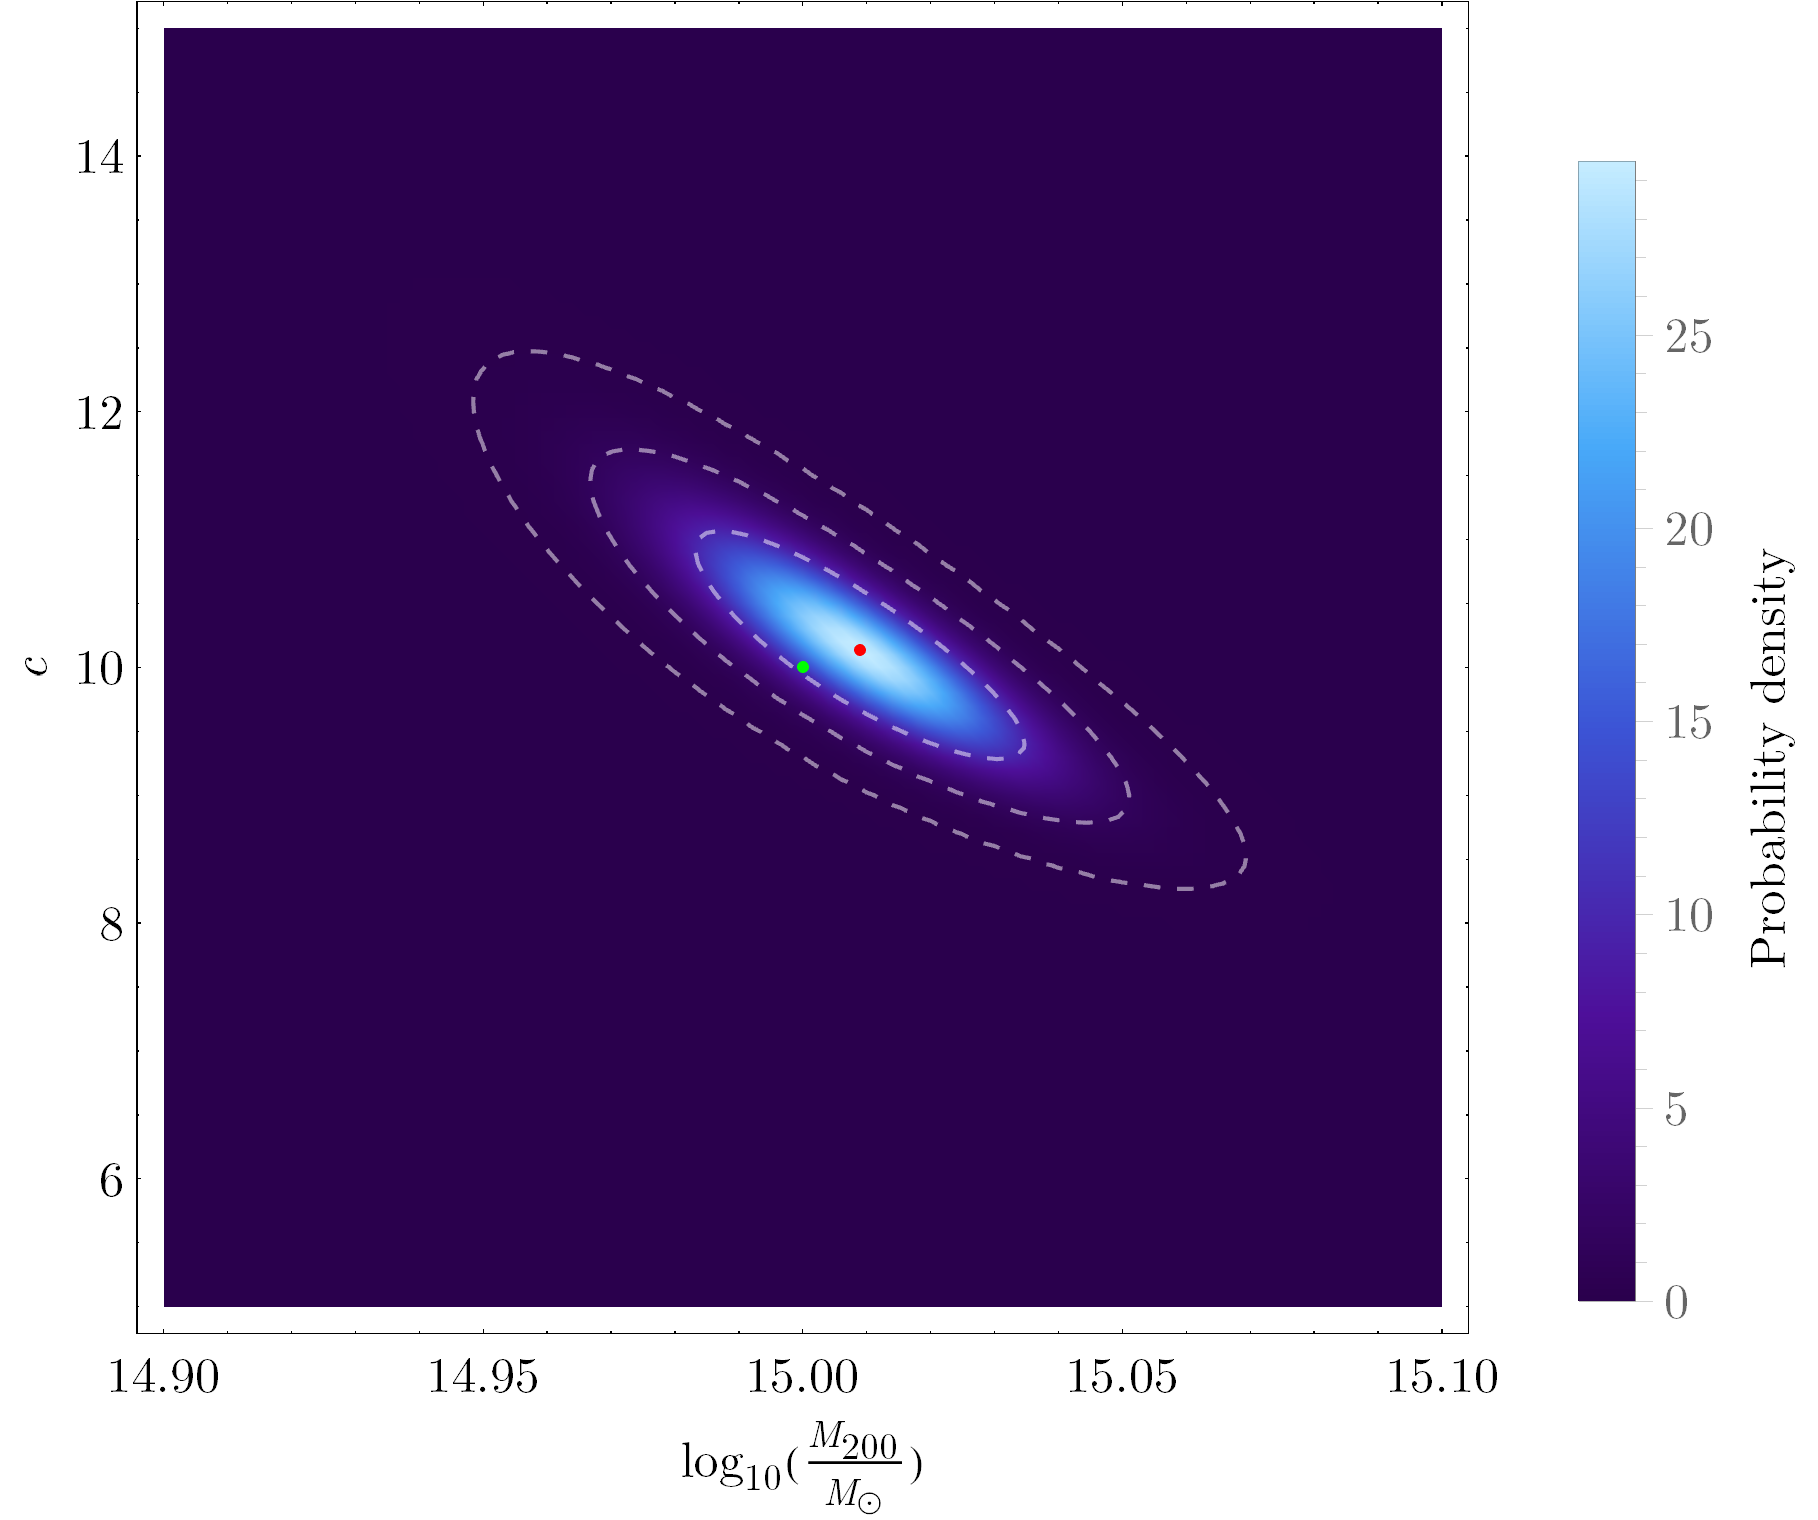
\includegraphics[width=0.49\textwidth]{nfwfitparams.pdf}
%     \caption{plots}
%     \label{}
% \end{figure}


\section{Conclusions}

Like (COMPARISONS BETWEEN ISOTHERMAL AND NFW MASS PROFILES
FOR STRONG-LENSING GALAXY CLUSTERS), we find that the strong lensing regime provides the most
But also, weak lensing can in fact provide sufficient distinguishability

has been applied to observations before
https://arxiv.org/pdf/astro-ph/9602053.pdf
but not in the context of comparing density profiles using for strong and weak
but this is highly dependent on good data

http://iopscience.iop.org/article/10.1086/590049/pdf looked at NFW vs isothermal in strong lensing with a focus on arcs, and found differing levels of distinguishibility for different lenses.

https://arxiv.org/pdf/1101.0650.pdf - our results don't match

may want to try fitting to CIS-generated data

Estimating ellipticity has well-documented issues [cite] due to noise and PSF


ignore cosmic shear (https://journals.aps.org/prd/pdf/10.1103/PhysRevD.70.023008)

From our data analysis, we were able to find the more probable density profile of a simulated data set.
Since the simulated data is based on the NFW and isothermal profile models, we were able to decisively distinguish between the two.
When analyzing real observed data, we expect the probability ratios to be relatively more even.
Future goals include the use of these methods to analyze observed data of galaxy clusters to find the density profile of their lenses.

%Where to go from here?


\bibliographystyle{aasjournal}
\bibliography{references}

\end{document}
